\documentclass[a4paper,12pt,twoside]{article}
\usepackage[utf8]{inputenc}
\usepackage{polski}
\usepackage{dirtree}
\usepackage{graphicx}
\usepackage{lastpage}
\usepackage{fancyhdr}
\newcommand\nazwa{"Eskulap" }

\pagestyle{fancy}
\renewcommand{\headrulewidth}{0pt}
\fancyhead{}
\cfoot{Strona\;\thepage\;z\;\pageref{LastPage}}

\title{SPECYFIKACJA FUNKCJONALNA \\ \nazwa}
\date{14 grudnia 2020}
\author{Piotr Nowak \\Hubert Piłka \\Dominik Wawrzyniuk}

\begin{document}

\maketitle
\tableofcontents

\section{Scenariusz projektu}
\nazwa ma na celu symulację transportu pacjentów do szpitali znajdujących się na terenie określonego obszaru. \nazwa zrealizuje to zadanie poprzez interfejs graficzny oraz zaimplementowany kod źródłowy.

\section{Użytkownicy projektu}
\nazwa jest przeznaczony zarówno dla kierowców karetek jak i pacjentów.

\section{Uruchomienie projektu}
\nazwa będzie uruchamiany poprzez maszynę wirtualną języka źródłowego. \nazwa nie wymaga żadnych parametrów wejściowych. Poniżej przedstawiono kod uruchamiający program w środowisku Command Line systemu operacyjnego Windows.

\paragraph{}
java \nazwa

\section{Funkcjonalność projektu}
\nazwa będzie spełniać szereg zadań wymaganych do poprawnej symulacji założonego scenariusza. Należą do nich:
\begin{itemize}
	\item Przedstawienie aktualnego stanu programu w interfejsie graficznym
	\item Czytanie podanego pliku wejściowego zawierającego informacje o szpitalach, obiektach i drogach
	\item Wykrycie przecinających się dróg i rozpatrzenie ich w scenariuszu
	\item Wyznaczenie oraz wyświetlenie obszaru państwa w interfejsie graficznym
	\item Wyświetlanie wybranych przez użytkownika kategorii konstrukcji: szpitale, obiekty, drogi
	\item Czytanie podanego pliku wejściowego zawierającego informacje o pacjentach
	\item Zwrócenie informacji dotyczącej błędów napotkanych w plikach wejściowych
	\item Dodawanie pacjenta poprzez wybranie miejsca w interfejsie graficznym lub przez podanie współrzędnych
	\item Ocena i informacja czy dany pacjent jest w granicach państwa
	\item Wypisywanie kolejnych przystanków trasy pacjenta
	\item Animacja trasy pacjenta
	\item Sterowanie szybkością programu
	\item Wyświetlanie ilości pacjentów, wolnych miejsc i długości kolejki w wybranym szpitalu
\end{itemize}

\section{Struktura projektu}
Główny folder projektu będzie nosił nazwę \nazwa. W nim zawarte będą cztery foldery o nazwach doc, build, src oraz test. Poniżej wymienione są zawartości poszczególnych folderów:
\begin{itemize}
	\item doc zawiera pliki tex, pdf oraz png dotyczące dokumentacji projektu.
	\item build zawiera skompilowane klasy potrzebne do uruchomienia projektu.
	\item src zawiera kod źródłowy projektu.
	\item test zawiera testy jednostkowe projektu.
\end{itemize}
Poniżej znajduje się schemat struktury projektu.
\dirtree{%
	.1 \nazwa.
	.2 doc.
	.2 build.
	.2 src.
	.2 test.
}

\section{Format danych wejściowych}
Program przyjmować będzie dwa pliki wejściowe:
\begin{enumerate}
	\item Plik zawierający informacje o szpitalach, obiektach i drogach
	\item Plik zawierający informacje o pacjentach
\end{enumerate}
Poniżej przedstawiono oczekiwany format pliku 1.\newline
\# Szpitale (id $|$ nazwa $|$ wsp. x $|$ wsp. y $|$ Liczba łóżek $|$ Liczba wolnych łóżek)\newline
1 $|$ Szpital Wojewódzki nr 997 $|$ 10 $|$ 10 $|$ 1000 $|$ 100\newline
...\newline
\# Obiekty (id $|$ nazwa $|$ wsp. x $|$ wsp. y)\newline
1 $|$ Pomnik Wikipedii $|$ -1 $|$ 50\newline
...\newline
\# Drogi (id $|$ id\_szpitala $|$ id\_szpitala $|$ odległość)\newline
1 $|$ 1 $|$ 2 $|$ 700\newline
...

\paragraph{}
Poniżej przedstawiono oczekiwany format pliku 2.\newline
\# Pacjenci (id $|$ wsp. x $|$ wsp.y)\newline
1 $|$ 20 $|$ 20\newline
...\newline

\paragraph{}
Linijki których pierwszy znak to hashtag (\#) są traktowane jako początek następnego bloku informacji. Pliki nie dostosowane do powyższych formatów nie zostaną poprawnie odczytane i program zwróci informację o napotkanym błędzie w trakcie czytania pliku.

\section{Format danych wyjściowych}
Program nie zwraca żadnych plików wyjściowych.

\section{Interfejs graficzny}
Interfejs graficzny składać się będzie z:
\begin{itemize}
	\item Narysowanego państwa wraz ze szpitalami, obiektami oraz drogami
	\item Guzików pozwalających na wczytanie plików wejściowych
	\item Slidera pozwalającego na regulowanie prędkości programu
	\item Formularza do wprowadzenia współrzędnych w których ma się pojawić pacjent
	\item Obszaru w którym wypisane będą kolejne przystanki transportowanego pacjenta oraz błędy
\end{itemize}
Dodatkowo za pomocą myszki będzie można również umieszczać pacjentów oraz sprawdzać ile pacjentów, wolnych miejsc oraz pacjentów w kolejce znajduje się w szpitalu pod myszką.

\section{Scenariusz użycia}
Poniżej znajduje się schemat blokowy scenariusza użycia programu.

\newpage
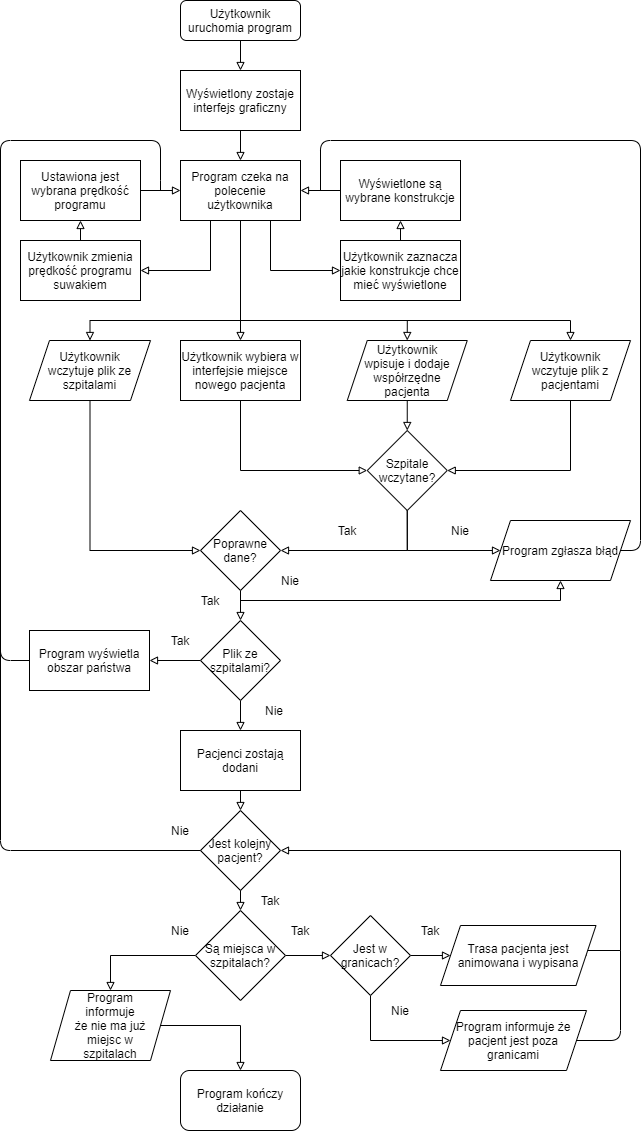
\includegraphics[width = \textwidth]{UserCase}

\section{Testowanie}
\nazwa zostanie przetestowany pod względem poprawności działania oraz wykrywania błędów w plikach wejściowych. Do przeprowadzenia testów zostanie użyte środowisko przeznaczone do testów jednostkowych.

\end{document}